\documentclass[a4paper,12pt]{article}
%%%%%%%%%%%%%%%%%%%%%%%%%%%%%%%%%%%%%%%%%%%%%%%%%%%%%%%%%%%%%%%%%%%%%%%%%%%%%%%%%%%%%%%%%%%%%%%%%%%%%%%%%%%%%%%%%%%%%%%%%%%%%%%%%%%%%%%%%%%%%%%%%%%%%%%%%%%%%%%%%%%%%%%%%%%%%%%%%%%%%%%%%%%%%%%%%%%%%%%%%%%%%%%%%%%%%%%%%%%%%%%%%%%%%%%%%%%%%%%%%%%%%%%%%%%%
\usepackage{eurosym}
\usepackage{vmargin}
\usepackage{amsmath}
\usepackage{graphics}
\usepackage{epsfig}
\usepackage{subfigure}
\usepackage{fancyhdr}
%\usepackage{listings}
\usepackage{framed}
\usepackage{graphicx}

\setcounter{MaxMatrixCols}{10}
%TCIDATA{OutputFilter=LATEX.DLL}
%TCIDATA{Version=5.00.0.2570}
%TCIDATA{<META NAME="SaveForMode" CONTENT="1">}
%TCIDATA{LastRevised=Wednesday, February 23, 2011 13:24:34}
%TCIDATA{<META NAME="GraphicsSave" CONTENT="32">}
%TCIDATA{Language=American English}

\pagestyle{fancy}
\setmarginsrb{20mm}{0mm}{20mm}{25mm}{12mm}{11mm}{0mm}{11mm}
\lhead{MA4128} \rhead{Kevin O'Brien}
\chead{Logistic Regression}
%\input{tcilatex}


\begin{document}

\section*{Model Metrics for Logistic Regression Models}
\begin{itemize}

\item In order to understand how much variation in the dependent variable can be explained 
by the model (the equivalent of $R^2$ in multiple regression), you should consult \textbf{\textit{Model Summary}} statistics.

\item Although there is no close analogous statistic in logistic regression to the coefficient of
determination $R^2$ the Model Summary Table provides some approximations.
\item 
Logistic regression does not have an equivalent to the R-squared that is found in OLS regression; however, many researchers have tried to come up with one. There are a wide variety of pseudo-R-squared statistics (of which we discuss only two).  Because this statistic does not mean what R-squared means in OLS regression (the proportion of variance explained by the predictors), interpreting this statistic must be done with great caution.
The pseudo-R-squared statistics will have lower values than in multiple regression


\item The SPSS output table below contains the \textit{Cox \& Snell R Square} and \textit{Nagelkerke R Square } values, which are both methods of calculating the explained variation.



\begin{figure}[h!]
	\centering
	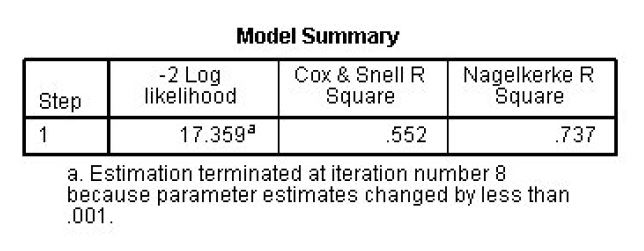
\includegraphics[width=0.9\linewidth]{images/Logistic5a}
\end{figure}



\item Cox and Snell’s R-Square is an attempt to imitate the interpretation of multiple R-squared based
on the likelihood, but its maximum can be (and usually is) less than 1.0, making it difficult to
interpret. 

\item Here it is indicating that 55.2\% of the variation in the Dependent Variable is explained by the
logistic model. 



%\item The Nagelkerke modification that does range from 0 to 1 is a more reliable measure of the relationship.



\item Nagelkerke's $R^2$ is part of SPSS output in the Model Summary table and is the most-
reported of the R-squared estimates. Nagelkerkes $R^2$ will normally be higher than the Cox and Snell measure.
\item In our case it is 0.737, indicating a moderately strong relationship of 73.7\% between the
predictors and the prediction.
\item Nagelkerke $R^2$ is a modification of Cox \& Snell $R^2$, the latter of which cannot achieve a value of 1. It is a enhancement of the Cox and Snell coefficient to assure that it can vary from 0 to 1. Nagelkerke's R-Square will normally be higher than the Cox and Snell measure. For this reason, it is preferable to report the Nagelkerke $R^2$ value.




\item  However, they are interpreted in the same manner, but with more caution. Therefore, the explained variation in the dependent variable based on this model ranges from 55.2\% to 73.7\%, depending on whether you reference the Cox \& Snell $R^2$ or Nagelkerke $R^2$ methods, respectively.

\end{itemize}

%%\begin{figure}[h!]
%%	\centering
%%	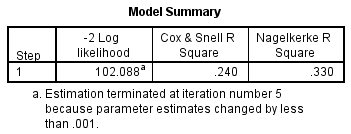
\includegraphics[width=0.9\linewidth]{images/BLogReg-Rsq}
%%	\caption{SPSS output}
%%	\label{fig:BLogReg-Rsq}
%%\end{figure}



\end{document}
